In this section, we evaluate the impact of approximations on the \gls{qoc} and memory of \gls{lkas}. 
First, we explain the scheduling of approximate \gls{isp} pipelines on \gls{gpu}.
Then, we perform both compute-centric and data-centric approximations. 

\subsection{Scheduling of approximate ISP pipelines on GPU}
\begin{figure}[ht]
    \centering
    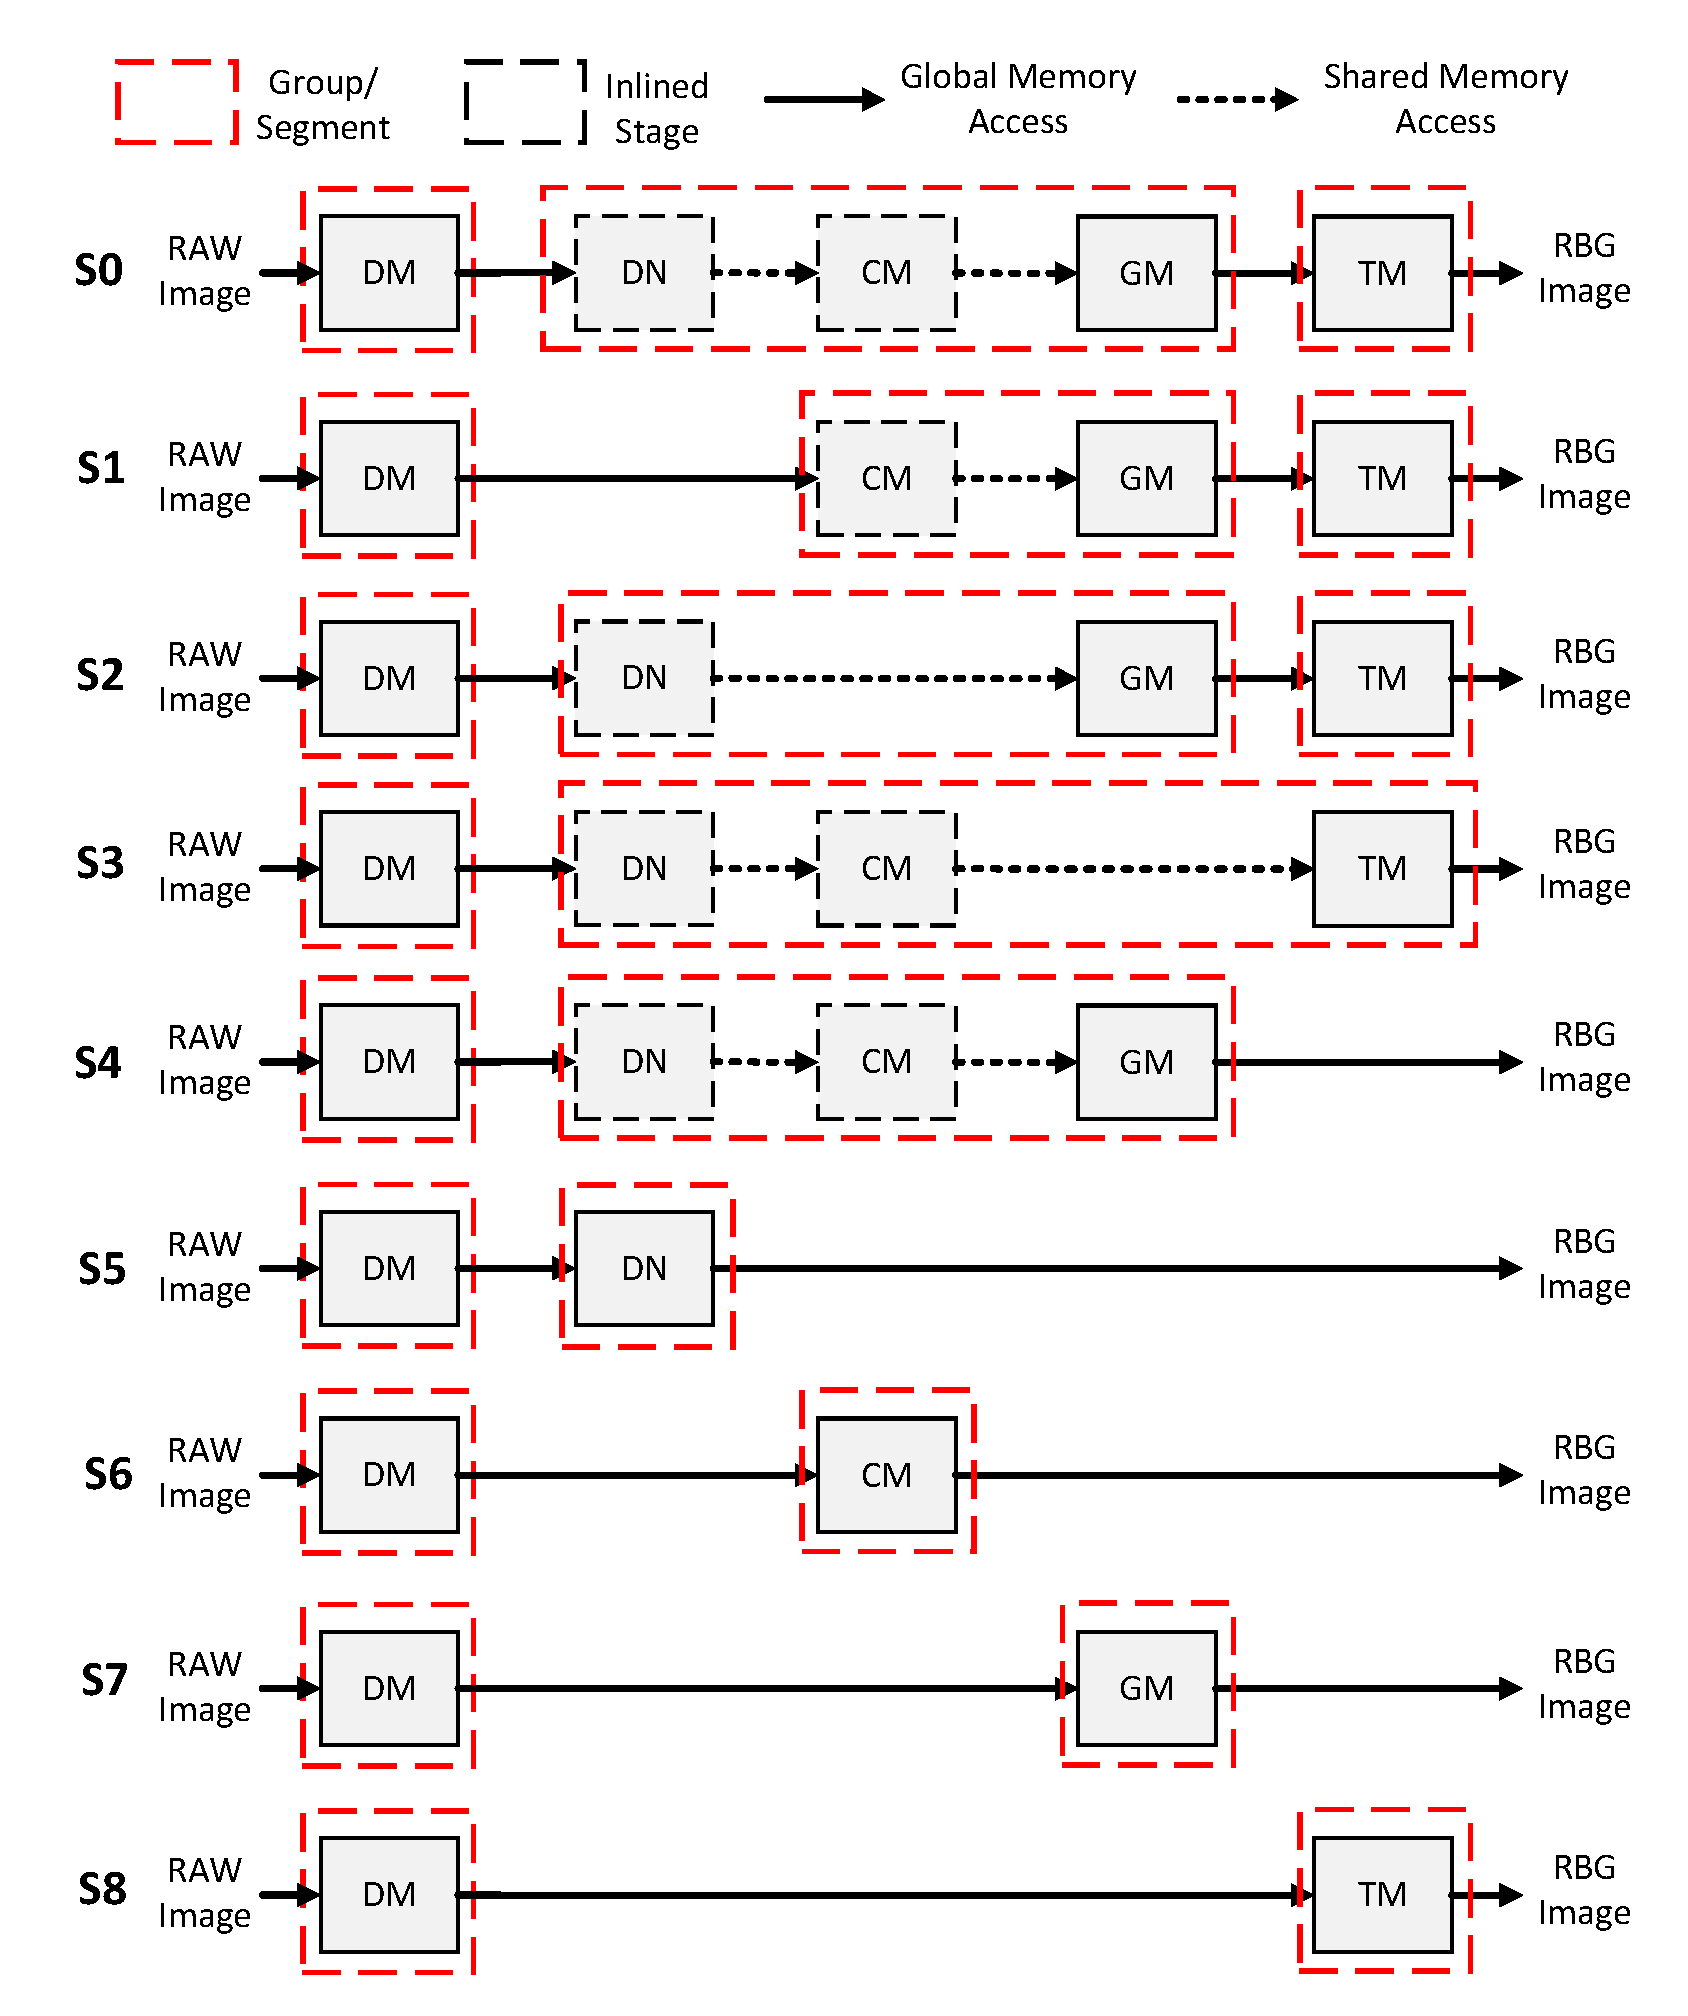
\includegraphics[width= 0.75\textwidth]{figs/isp_schedules.pdf}
    % \vspace{-5pt}
    \caption{{GPU schedules obtained for the different pipelines.}}
    \label{fig:gpu_sched}
    % \vspace{-10 pt}
\end{figure}
Execution time of different \gls{isp} pipeline settings depends on how they are scheduled on the GPU.  To generate optimized schedules, we use the Halide GPU auto-scheduler proposed in \cite{halide-auto}. The cost function of this auto-scheduler optimizes a pipeline by splitting it into groups/segments so that each segment can be executed with accesses to the GPU shared memory only. Also, each segment corresponds to a different CUDA kernel. When moving from one segment to another, we need accesses to the global memory. It should be noted that accesses to the global memory are orders of magnitude more costly compared to the ones to shared memory since DRAM bandwidth is often much lower than the bandwidth achieved by shared memory \cite{halide-auto}. That’s why the execution time of these pipeline settings highly depends on the number of global memory accesses.

We consider nine different pipeline settings, S0-S8. S0 is the fully accurate \gls{isp} pipeline; the other eight pipelines are approximated by skipping various stages, as further elaborated in the following subsection.
Fig.\ \ref{fig:gpu_sched} shows the GPU schedules we obtain for the different pipeline settings using the auto-scheduler \cite{halide-auto}. For splitting the pipelines into segments, the auto-scheduler starts from the output stage and continuously merges it with the previous stages as long as the data can be fit into the shared memory. If not, then it splits the pipeline into two segments and starts the same process again in the non-visited segment. The following observations are made from the schedules:
\begin{figure}[t]
    \centering
		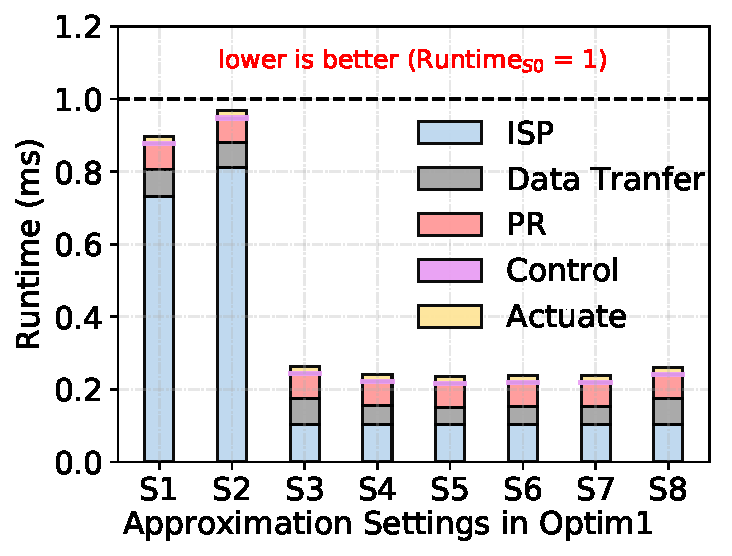
\includegraphics[width=0.6\textwidth]{figs/qoc_wtime_CPU_ALL_GPU2.pdf}
		\vspace{-7pt}
		\captionsetup{width=\textwidth}
		\caption{{Improvements in runtime from coarse-grained \gls{isp} approximation.}}
		\label{fig:qoc_runtime}
		\vspace{-9pt}
\end{figure}
\begin{itemize}
    \item Gamut mapping (GM) and tone mapping (TM) cannot be put into a single segment as the data cannot fit in shared memory. So, TM is put in a separate segment in S0-S2.
    \item The output of demosaicing (DM) has a high memory footprint. So, DM cannot be put in a single segment with the subsequent stages. This results in a separate segment for DM in S0-S8.
    \item The auto-scheduler prioritizes inlining of cascaded stages (within a segment) into the consumer, which maximizes  producer-consumer locality.
\end{itemize}

Fig.\ \ref{fig:qoc_runtime} shows the runtimes of the eight pipeline settings. We observe from Fig.\ \ref{fig:gpu_sched}, that settings S0-S2 have three segments/groups accessing the global memory while the rest, S3-S8, has two segments/groups accessing the global memory. This explains the higher execution time of S0-S2 compared to S3-S8 in Fig.\ \ref{fig:qoc_runtime}. This also explains why S3 and S4 (each with four stages) take the same time as S5-S8 (each with two stages). Also, the execution time does not scale linearly with the number of stages in the pipeline, which explains why all of S5-S8 combined seems to take less time than S0 (or S1 and S2) despite having more stages (as DM is common to all of them). It should be noted that the slight runtime variations in S0-S2 are due to extra thread synchronization overheads introduced by intra-segment communication through shared memories. The same reasoning applies to S3-S8.

\begin{table}[ht]
	\small
	\renewcommand{\arraystretch}{1.1}
	\caption{{Coarse-Grained Approximation Settings in Optim 1.}}
	\label{table_2}
	\centering
	\begin{threeparttable}	
		\setlength\tabcolsep{1pt}
		\begin{tabular}{>{\centering\arraybackslash}p{8mm}>{\centering\arraybackslash}p{38mm}>
				{\centering\arraybackslash}p{38mm}}
			\hline
			\hline
			\textbf{Setting} & \textbf{\gls{isp} Stages} &\textbf{Description} \\
			\hline
			S0 & DM, DN, CM, GM, TM  & Accurate (all stages included) \\
			\hline
			S1 & DM, CM, GM, TM  & Skip Denoising \\
			\hline
		    S2 & DM, DN, GM, TM  & Skip Color Mapping \\
			\hline
			S3 & DM, DN, CM, TM  & Skip Gamut Mapping \\
			 \hline
			S4 & DM, DN, CM, GM  & Skip Tone Mapping \\
			 \hline
			S5 & DM, DN  & Keep only Denoising \\
			\hline
			S6 & DM, CM  & Keep only Color Mapping \\
			\hline
			S7 & DM, GM  & Keep only Gamut Mapping \\
			\hline
			S8 & DM, TM  & Keep only Tone Mapping \\
			\hline
		\end{tabular}
		\begin{tablenotes}
			\footnotesize
			\item{DM: Demosaic, DN: Denoise, CM: Color Mapping, \\ GM: Gamut Mapping, TM: Tone Mapping} 
			\item{Note: We refer to S0 as the accurate setting as no stages are skipped. In the other (approximate) settings, S1-S8, certain stages are skipped.}
		\end{tablenotes}
	\end{threeparttable}
\end{table}

\begin{figure}[ht]
    \centering
    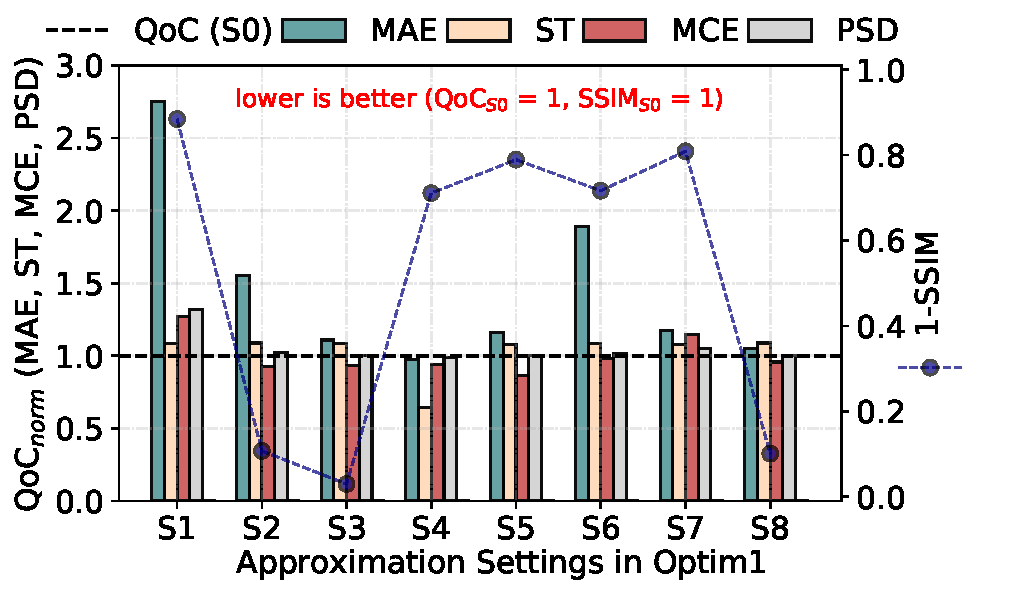
\includegraphics[width=0.8\textwidth]{figs/qoc_wotime_CPU_ALL_GPU1.pdf}
		\captionsetup{width=\linewidth}
		\caption{{\Gls{qoc} compared with image quality for different approximation settings. \gls{lkas} is operated in approximation-only mode with default settings (Section~\ref{metrics}).}}
		\label{fig:qoc_wotime}
\end{figure}  


\begin{figure}[thb]
    \centering
		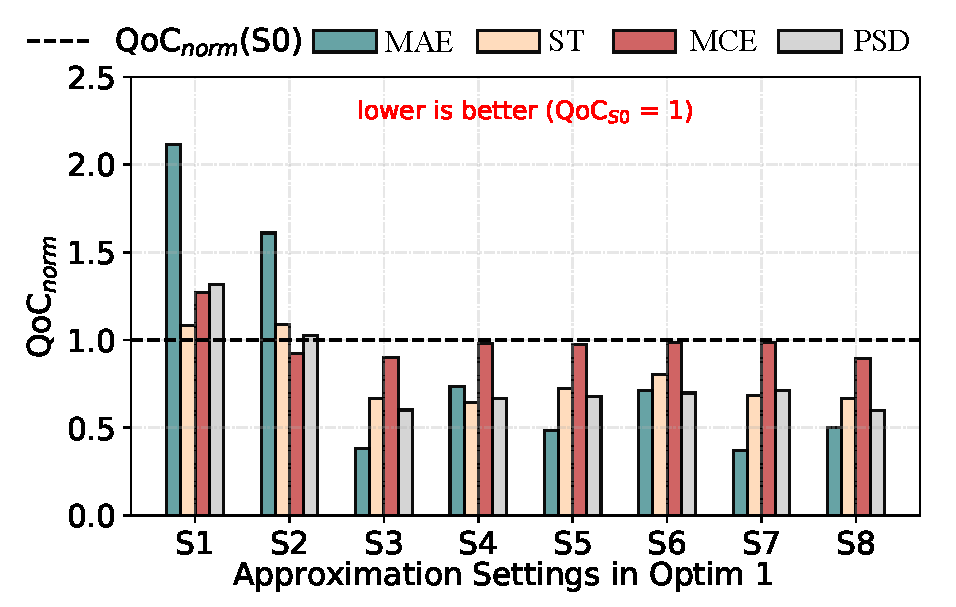
\includegraphics[width=0.8\textwidth]{figs/qoc_wtime_CPU_ALL_GPU1_2.pdf}
		\captionsetup{width=\linewidth}
		\caption{{\Gls{qoc} improvements with reduced sampling period. \gls{lkas} is operated in \gls{qoc}-optimal mode with default settings.}}
		\label{fig:qoc_wtime}
\end{figure}  

\subsection{Optim 1: coarse-grained \gls{isp} approximations}\label{ss_optim_1}
As mentioned, the \gls{isp} is approximated in a coarse-grained manner by skipping one or more sub-stages within the pipeline (see Fig.\ \ref{fig:isp}~(a)). Testing all possible combinations for skipping sub-stages is not feasible due to high compute overheads. So, for our analysis, we consider nine different approximation settings, as shown in Table~\ref{table_2}. Settings S1-S4 are obtained by skipping one stage at a time, while settings S5-S8 are obtained by keeping one stage and disabling the rest of the pipeline. It is noticed that skipping the DM stage results in an \gls{lkas} failure. This is because \gls{pr} algorithms operate in the RGB domain and they do not work for the Bayer domain. So, DM is essential for proper \gls{lkas} operation. Additionally, it needs to be mentioned that certain approximation settings initially led to \gls{lkas} failure. Minor modifications to the \gls{pr} stage to handle these errors made it working (as further explained in Section~\ref{sub_stages}). 

\par Skipping one or more sub-stages in the \gls{isp} has both positive and negative impacts on the \gls{qoc} of \gls{lkas}. The loss in image quality due to approximation settings (S1-S8) may degrade the \gls{qoc}. However, the reduced sensing-to-actuation delay ($\tau$) allows faster sampling of the controller, thereby improving the \gls{qoc}. Balancing this interaction is essential in determining if we gain or lose in final \gls{qoc}. We evaluate the former by operating \gls{lkas} in approximation-only mode (without considering faster sampling) and the latter by operating \gls{lkas} in \gls{qoc}-optimal mode (considering faster sampling).

\par Fig.~\ref{fig:qoc_wotime} shows a comparison between image degradation and \gls{qoc} of \gls{lkas}. The \gls{qoc} metrics (\gls{mae}, \gls{st}, \gls{mce} and \gls{psd}) on the left x-axis are normalized to the accurate setting (S0). The \gls{ssim} loss (right y-axis) shows the degree of image degradation. First, it is evident that the different settings (S1-S8) have varying impact on image quality. S1 (skipping denoising DN) performs the worst in terms of both image quality and \gls{qoc}. We conclude that skipping DN while keeping the rest of the stages (S1) is not a suitable candidate for getting better \gls{qoc}. We also observe that some settings (S3, S4, S5, S7, S8) perform relatively similar to the baseline. This shows that \gls{isp} pipelines optimized for human vision are overkill for \gls{lkas}. There is no one-to-one correlation between image degradation and \gls{qoc}. For instance, settings S4, S5 and S7 have high \gls{ssim} loss (more degradation) but they perform similar to S0 in terms of \gls{qoc}, with S4 being slightly better. Contrarily, S2 has low \gls{ssim} loss but high \gls{mae} (worse \gls{qoc}). This is explained by the fact that the performance of control algorithms depends on the presence of an essential feature in the image (lane markings in this case). Image-degradation metrics like \gls{ssim} loss fail to identify this. This non-correlation shows that approximating different subsystems individually without considering the impact on the bigger closed-loop system can lead to sub-optimal results.  

\par Fig.~\ref{fig:qoc_runtime} shows that lowered compute workloads due to approximations (S1-S8) result in up to 76\% reduction (S5) in the sensing-to-actuation delay ($\tau$). This allows faster sampling of the controller. This is taken into account in Fig.\ \ref{fig:qoc_wtime} that shows the \gls{qoc} for the nine pipeline settings. We observe a significant impact of reduced sampling period on the \gls{qoc}. Faster control sampling in S3-S8 due to reduced $\tau$ overshadows the negative impact of image degradation on \gls{qoc}. We observe up to 63\% (S7), 35\% (S4), 10\% (S8), 40\% (S8) improvements in \gls{mae}, \gls{st}, \gls{mce} and \gls{psd} respectively. However, in settings S1 and S2, the minor reductions in $\tau$ do not allow a faster sampling. So, the negative impact of image degradation is not balanced, resulting in worsened \gls{qoc}. From Fig.\ \ref{fig:qoc_wotime}, we observe that skipping only gamut mapping (S3) and keeping only gamut mapping (S7) have opposite impacts on the visual quality of the image. However, both S3 and S7 have minimal effects on the essential features (lane markings) of the image \cite{buckler}. This is evident in Fig.\ \ref{fig:qoc_wtime} where both settings S3 and S7 perform similarly in terms of \gls{qoc} (0.38 and 0.36 respectively) with S7 being slightly better than S3. 
Fig. \ref{fig:memory_optim1} reports the memory improvements in \gls{lkas} due to Optim 1. Up to 69\% reduction (S5) in memory traffic is obtained from Optim 1.

\begin{figure}[ht]
\centering
\begin{subfigure}{0.39\textwidth}
\centering
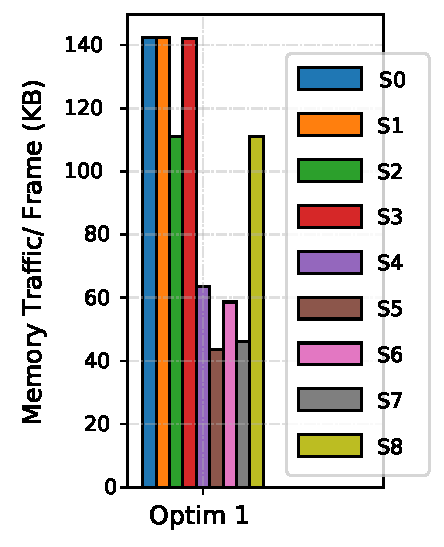
\includegraphics[width=\textwidth]{figs/memory_CPU_ALL_GPU.pdf}
		\captionsetup{width=\linewidth}
		\caption{{Memory traffic reduction due to Optim 1.}}
		\label{fig:memory_optim1}
\end{subfigure}
\begin{subfigure}{0.59\textwidth}
\centering
	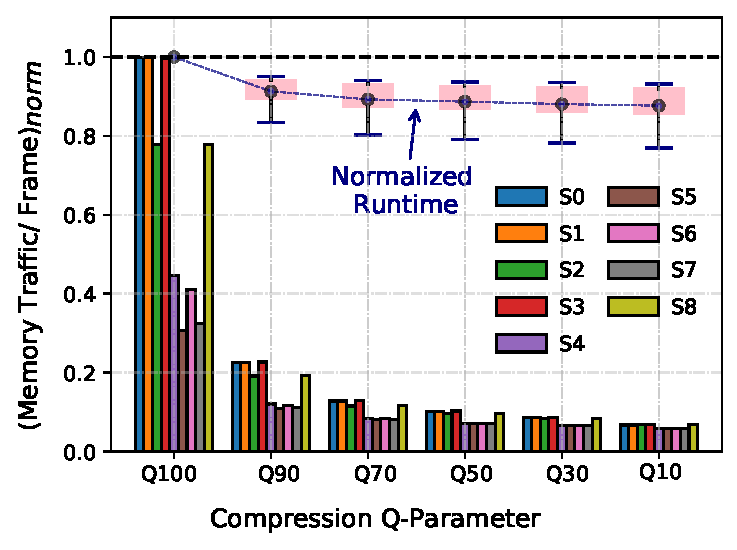
\includegraphics[width=\textwidth]{figs/robustness3_1.pdf}
		\captionsetup{width=0.8\textwidth}
		\caption{{Off-chip memory traffic reduction and runtime improvements from variable Q-parameter (Optim 2).}}
		\label{fig:optim2_1}
\end{subfigure}
\caption{Memory traffic reductions}
\label{fig:combined}
\vspace{-2em}
\end{figure}

\subsection{Optim 2: lossy compression using variable Q-parameter}\label{ss_optim2}
\par As a next step, we vary the Q-parameter in the JPEG algorithm to control the degree of lossy compression to reduce the off-chip memory traffic. In the evaluation of Optim 1, a fixed Q-parameter ($=$ 100) was considered. For Optim 2, the Q-parameter is modulated in fixed steps from Q10 to Q90 in addition to Q100. Fig.\ \ref{fig:optim2_1} shows the off-chip memory traffic reduction for the different approximation settings while varying the Q-parameter. All values are normalized to S0\textsub{Optim 1}. S5 is the most memory-efficient setting across all Q-parameters. For S5, additional memory reductions of up to 81\% (Q10) are obtained over Optim 1. However, these reductions come at a cost; they introduce more noise to the system. To gain on \gls{qoc} for the entire system, there must be significant runtime reductions in $\tau$ to allow for faster control sampling. We observe that for lower values of Q (Q $<$ 70), the additional runtime reductions are insignificant (see Fig.\ \ref{fig:optim2_1}). Lower Q-parameter values lead to more aggressive quantization during compression. However, for smaller pixel values (more common in approximated images), values are rounded to zero resulting in no additional reduction in memory traffic, and thereby no runtime improvements. So, we consider only higher values of Q ($\geq$ 70).

\subsection{Interstage effects of approximations}\label{sub_stages}
It is observed that both the coarse-grained approximations in Optim 1 and the lossy compression in Optim 2, have a quality impact on the subsequent stages, especially the \gls{pr} stage. However, the impact of Optim 1 on the \gls{pr} stage is critical, as it results in \gls{lkas} failure in some cases. The \gls{pr} stage does not detect the lanes properly for certain approximated streams obtained from S1-S8. The problem is traced back to the static image thresholding step in \gls{pr} (see Fig.~\ref{fig:isp}~(b)), which fails to identify the lane markers from the grayscale bird's eye view image due to incorrect choice of threshold. To counter this, Otsu's binarization algorithm is used, which dynamically identifies the optimal threshold. Otsu's algorithm brings an additional computational complexity of $MN + 7L^2+5L-12$, for an $M \times N$ image with $L$ grey levels. Depending on the approximation settings, dynamic thresholding is either performed on the grayscale bird's eye view image or RGB bird's eye view image. This results in desired \gls{lkas} behaviour across all approximation settings. It is noted that performing dynamic thresholding on the RGB image has thrice the computational complexity, which has been taken into account in our evaluation results.